\documentclass[twoside]{article}

%/Network/Applications/texmaker.app/Contents/MacOS/../Resources/en_US.dic
%/usr/local/macports108/bin/latex

\usepackage{amsmath,amssymb,graphicx}
\usepackage[ngerman]{babel}
\usepackage{graphics}
\usepackage{graphicx}
\usepackage{float}
\usepackage{floatflt}
\usepackage{rotating}

\usepackage{hyperref}

\setlength{\parindent}{0pt} 


\usepackage{xcolor}
\usepackage{cite}
\usepackage{amsmath,amssymb,amsbsy,amsfonts,amsthm,amstext}
%\usepackage{anysize}
%\usepackage[margin=12pt,labelfont=bf, format=hang, justification =raggedright]{subcaption}%font=scriptsize
\usepackage[margin=12pt,labelfont=bf, labelsep=endash, format=hang, justification =raggedright]{caption}
%\usepackage{titlesec}
%\titleformat*{\section}{\large\bfseries}
%\titleformat*{\subsection}{\normalsize\bfseries}
%\titleformat*{\subsubsection}{\normalsize\bfseries}

\newcommand{\eg}{\textit{e.g.~}}
\newcommand{\ie}{\textit{i.e.~}}
\newcommand{\etal}{\textit{et al.~}}
\newcommand{\wrt}{\textit{w.r.t.~}}
\newcommand{\cf}{\textit{cf.~}}
\newcommand{\comment}[1]{\textcolor{red}{\noindent\bfseries #1}}
%------------------------------------------------------------
\begin{document}

%%%%%%%%% TITLE of abstract %%%%%%%%%

\begin{center}
\textbf{\Large Komplexes Kompartiment Modell f\"ur die Corona Pandemie}
\end{center}

%\medskip

%%%%%%%%%  AUTHORS %%%%%%%%%

\begin{center}
Birte Schmidtmann\\%$^{a}$, Eva Oellingrath$^a$, Mirko Himmel$^a$\\
{\small{%${}^a$ 
\emph{Zentrum f\"ur Naturwissenschaft und Friedensforschung (ZNF), Universit\"at Hamburg, Bogenallee 11, 20144 Hamburg}}}
%\texttt{schmidtmann@mathcces.rwth-aachen.de}
\end{center}

%\keywords{Norovirus, Germany, federal state, Weather}
%novel scientific contribution of this work: 

\bigskip

%%%%%%%%%  text of ABSTRACT to be included below  %%%%%%
%	\begin{abstract}
%	bla
%	\end{abstract}
	%
%==============================
\section{Das Modell}\label{sec:modell}
%==============================	
%
In diesem Kompartiment Modell wird die Bev\"olkerung in die folgenden Gruppen (Kompartimente) aufgeteilt:\\
\begin{itemize}
\item $S$: Susceptible. Gesunde Personen, die gegen die Krankheit nicht immun sind.
\item $L$: Latent. Bereits infizierte Personen ohne Symptome. Im Fall von SARS-CoV-2 sind diese Personen infekti\"os, k\"onnen das Virus also unwissentlich weiter verbreiten. Die Ansteckungswahrscheinlichkeit von suszeptiblen Personen durch eine latente Person ist hoch.
\item $I_m$: infected mild. Infizierte Personen mit milden Symptomen.
\item $I_s$: infected severe. Infizierte Personen mit starken Symptomen.
\item $H$: hospitalized. Infizierte Personen, die im Krankenhaus ist.
\item $ICU$: intensive care unit. Infizierte Personen, die im Krankenhaus auf der Intensivstation liegt.
\item $R$: recovered. Genesene Personen.
\item $D$: deceased. An der Krankheit verstorbene Personen.
\item $Q$: quarantined. Personen in Heim-/Selbst-Isolation oder in  Quarant\"ane.
\end{itemize}
%
\begin{figure}[h!]
	\centering
	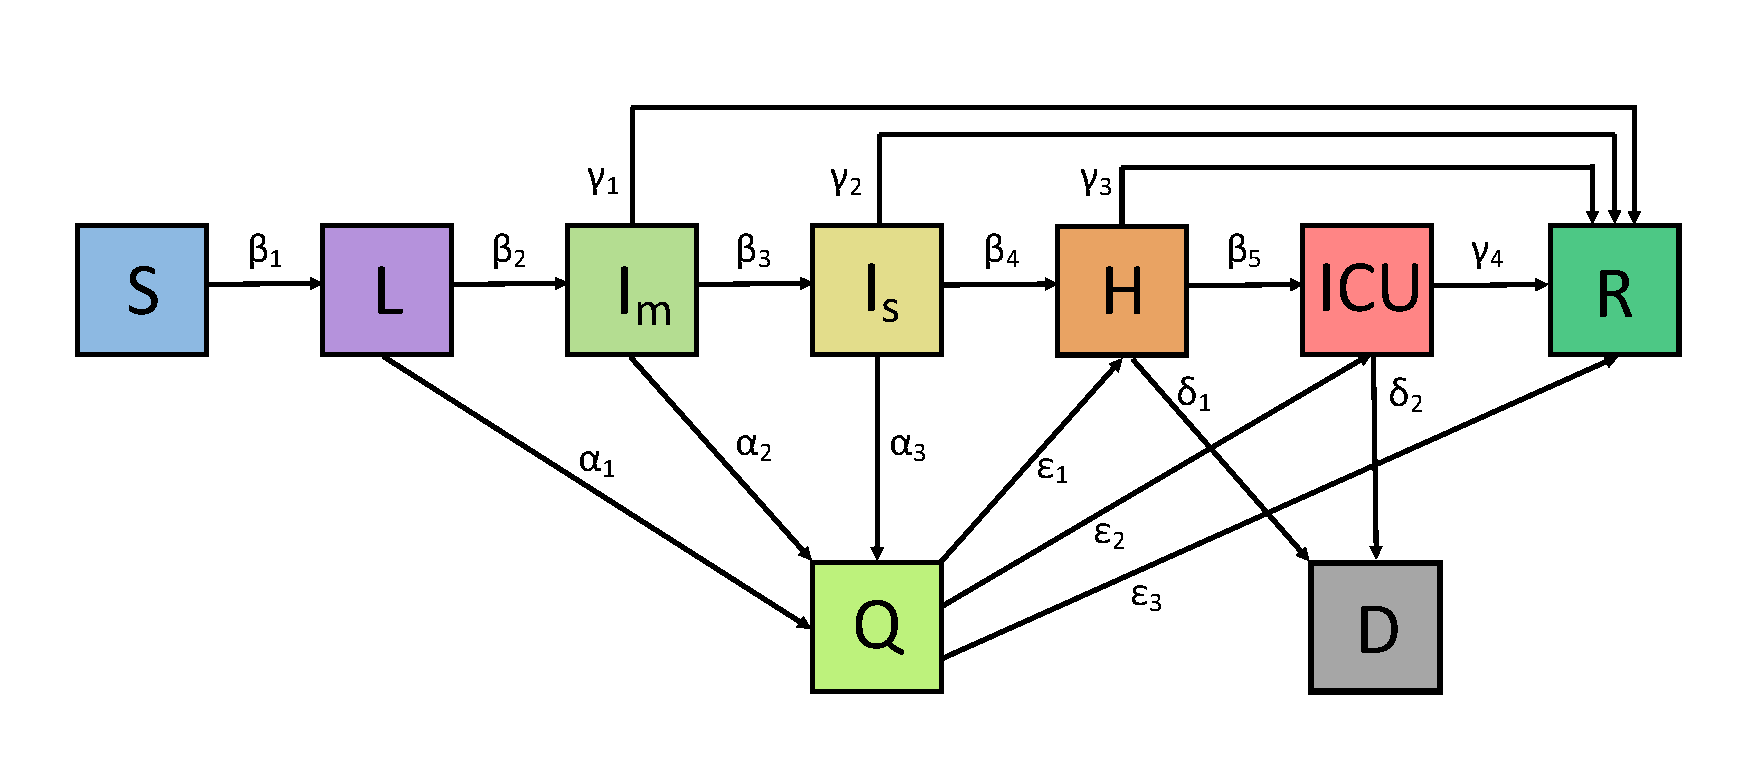
\includegraphics[width=\textwidth]{./flowchart.pdf}
\end{figure}
%
In diesem Modell sind die Raten $\beta_i,\;i=1,\ldots,5, \gamma_j,\;j=1,\ldots,4,
\alpha_k, \varepsilon_k, \;k=1,\ldots,3$ und $\delta_\ell,\;\ell=1,2$ enthalten. Diese Raten sind entscheidend daf\"ur, wie viele Menschen pro Zeiteinheit zwischen den Kompartimenten wechseln.

Die sogenannte attack rate oder infection rate $\beta_1$ kann man sich vorstellen, als die Rate mit der infizierte Personen krankheits\"ubertragende Kontakte haben. Multipliziert man diese Rate mit der Anzahl latenter Personen zum Zeitpunkt $t$ (die zum Gro\ss teil nicht wissen, dass sie infiziert sind) erh\"alt man die Gesamtrate krankheits\"ubertragender Kontakte pro Zeiteinheit $\beta_1 L(t)$. Da nur der Teil $S(t)/N$ aller vorkommenden Kontakte immunologisch naiv f\"ur die Krankheit ist, finden $\beta_1 L(t)S(t)/N$ Krankheits\"ubertragungen statt. 
Da nicht nur infizierte Personen ohne Symptome ($L$) das Virus weiter verbreiten k\"onnen, sondern auch mild infizierte ($I_m$), infizierte mit starken Symptomen ($I_s$), Personen im Krankenhaus ($H$ und $ICU$), die Pflegepersonal und \"ArztInnen anstecken k\"onnen, sowie heimisolierte Personen ($Q$), die Familienmitglieder anstecken k\"onnen, wird der Term $\beta_1 S(t)/N$ mit einer gewichteten Summe dieser Kompartimente multipliziert. Durch die Vorfaktoren $\kappa_m, \kappa_s, \kappa_H, \kappa_{ICU}, \kappa_Q$ kann die Rate krankheits\"ubertragender Kontakte f\"ur jeden Personenkreis angepasst werden. Zum Beispiel wird die Ansteckungsrate isolierter Personen niedriger sein, als die Rate hospitalisierter oder latenter.\\
{\ }\\
Die recovery rate $\gamma_i$ gibt an, wie viele Zeiteinheiten man braucht, um zu genesen. Diese Rate unterscheiden sich f\"ur die Gruppen $I_m, I_s, H$ und $ICU$. Es wird davon ausgegangen, dass latente Personen entweder in die Prodromalphase mit milden Symptomen \"ubergehen oder getestet werden und sich in Quarant\"ane begeben. Einen \"Ubergang von latent zu recovered ist nicht vorgesehen, da ein symptomfreier Krankheitsverlauf als sehr unwahrscheinlich gilt \cite{1}.

bisher habe ich folgende Raten verwendet:\\
$\beta_1 = 3.0$ \\
$\beta_2 = 0.3$ \\
$\beta_3 = 0.3$ \\
$\beta_4 = 0.1$ \\
$\beta_5 = 0.05$ \\
$\gamma_1 = 1./3$ \\
$\gamma_2 = 1./3$ \\
$\gamma_3 = 1./3$ \\
$\gamma_4 = 1./3$ \\
$\alpha_1 = 0.2$ \\
$\alpha_2 = 0.5$ \\
$\alpha_3 = 0.2$ \\
$\varepsilon_1 = 0.2$ \\
$\varepsilon_2 = 0.1$ \\
$\varepsilon_3 = 0.7$ \\
$\delta_1 = 0.01$ \\
$\delta_2 = 0.05$ \\
$\kappa_m = 0.8$ \\
$\kappa_s = 0.2$ \\
$\kappa_H = 0.2$ \\
$\kappa_ICU = 0.1$ \\
$\kappa_Q = 0.01$.

Die dazugeh\"origen Formeln lauten 
\begin{align*}
\frac{d S}{dt} &= -\beta_1 \frac{S(t)}{N}\left( L(t) + \kappa_m I_m(t)+ \kappa_s I_s(t) + \kappa_H H(t) + \kappa_{ICU} ICU(t) + \kappa_Q Q(t)\phantom{\frac{.}{.}}\right)\\
%
\frac{d L}{dt} &= +\beta_1 \frac{S(t)}{N}\left( L(t) + \kappa_m I_m(t)+ \kappa_s I_s(t) + \kappa_H H(t) + \kappa_{ICU} ICU(t) + \kappa_Q Q(t)\phantom{\frac{.}{.}}\right) - \beta_2 L(t) - \alpha_1 L(t)\\
%
\frac{d I_m}{dt} &= +\beta_2 L(t) - \beta_3 I_m(t)- \gamma_1 I_m(t)-\alpha_2 I_m(t)\\
%
\frac{d I_s}{dt} &= +\beta_3 I_m(t) - \beta_4 I_s(t) - \gamma_2 I_s(t) - \alpha_3 I_s(t) \\
%
\frac{d H}{dt} &= +\beta_4 I_s(t) + \varepsilon_1 Q(t) - \beta_5 H(t) - \gamma_3 H(t) - \delta_1 H(t)\\
%
\frac{d ICU}{dt} &= +\beta_5 H(t) + \varepsilon_2 Q(t) - \gamma_4 ICU(t) - \delta_2 ICU(t)\\
%
\frac{d R}{dt} &= +\gamma_1 I_m(t)+\gamma_2 I_s(t)+\gamma_3 H(t) +\gamma_4 ICU(t) +\varepsilon_3 Q(t) \\
\frac{d D}{dt} &= +\delta_1 H(t) + \delta_2 ICU(t)\\
%
\frac{d Q}{dt} &= +\alpha_1 L(t) + \alpha_2 I_m(t) + \alpha_3 I_s(t) - \varepsilon_1 Q(t)- \varepsilon_2 Q(t)- \varepsilon_3 Q(t)
%
\end{align*}

und die Ergebnisse ohne Pendlerdaten und ohne Ma\ss nahmen wie Kontaktsperren oder Selbstisolierung im gro\ss en Stil (wie wir sie im Moment praktizieren) sind in Abb. \ref{fig:ersteErgebnisse} und \ref{fig:ersteErgebnisseZoom} zu sehen. 
%
\begin{figure}[h!]
	\centering
	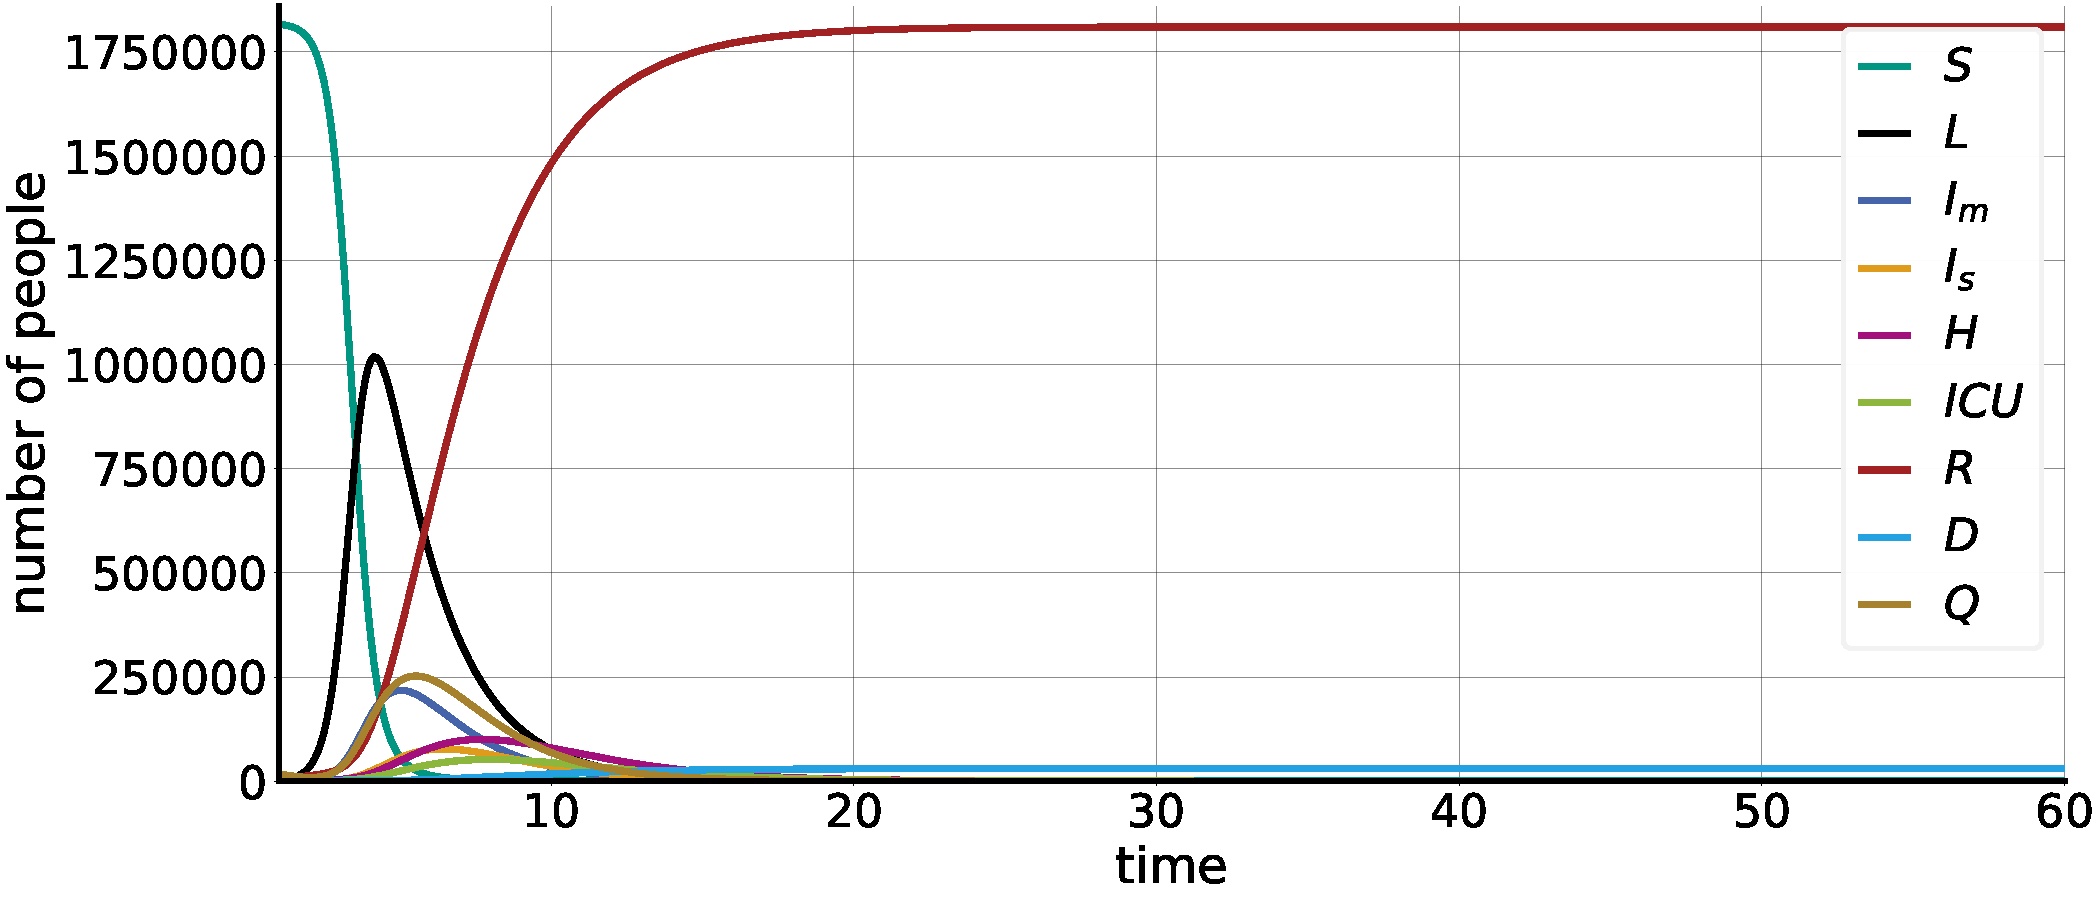
\includegraphics[width=\textwidth]{./hamburgSIR}
	\caption{Erste Ergebnisse.}
	\label{fig:ersteErgebnisse}
\end{figure}
%
\begin{figure}
	\centering
	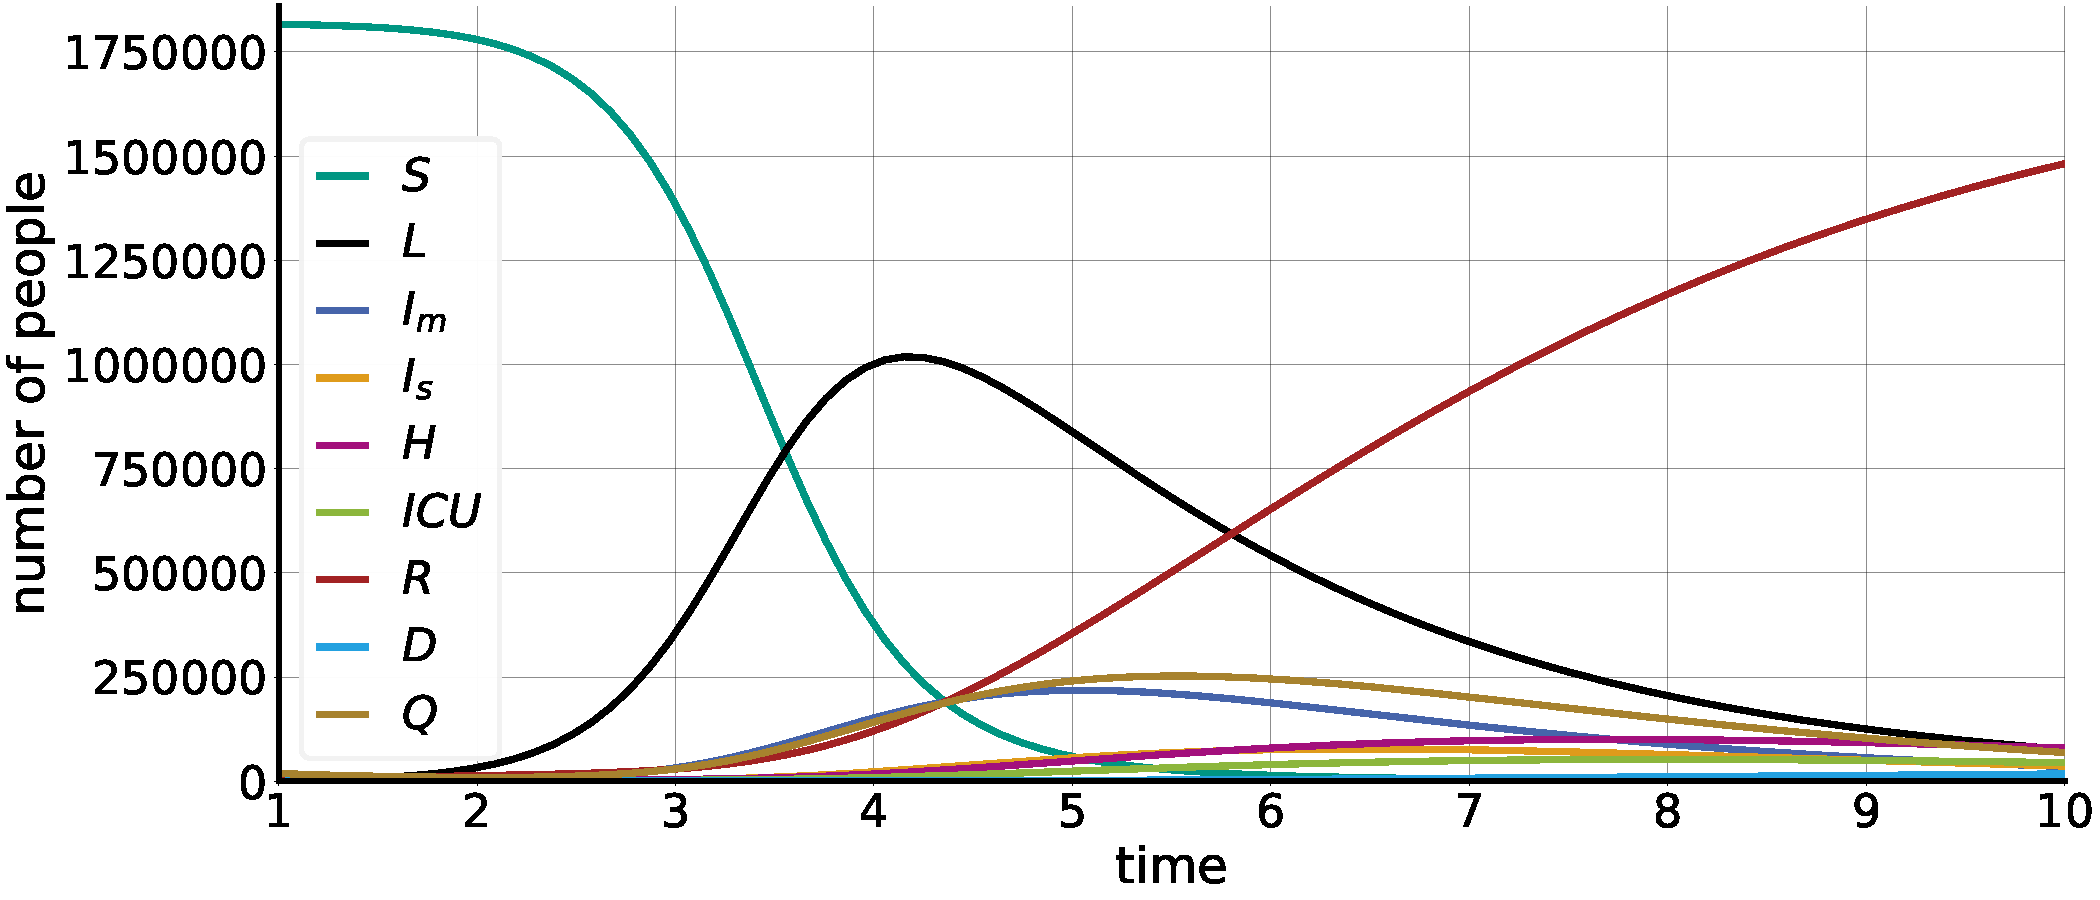
\includegraphics[width=\textwidth]{./hamburgSIRzoom}
	\caption{Erste Ergebnisse, zoom.}
	\label{fig:ersteErgebnisseZoom}	
\end{figure}


Im Folgenden sollen einige Pendler hinzukommen, siehe \ref{fig:modellPendler}
\begin{figure}[h!]
	\centering
	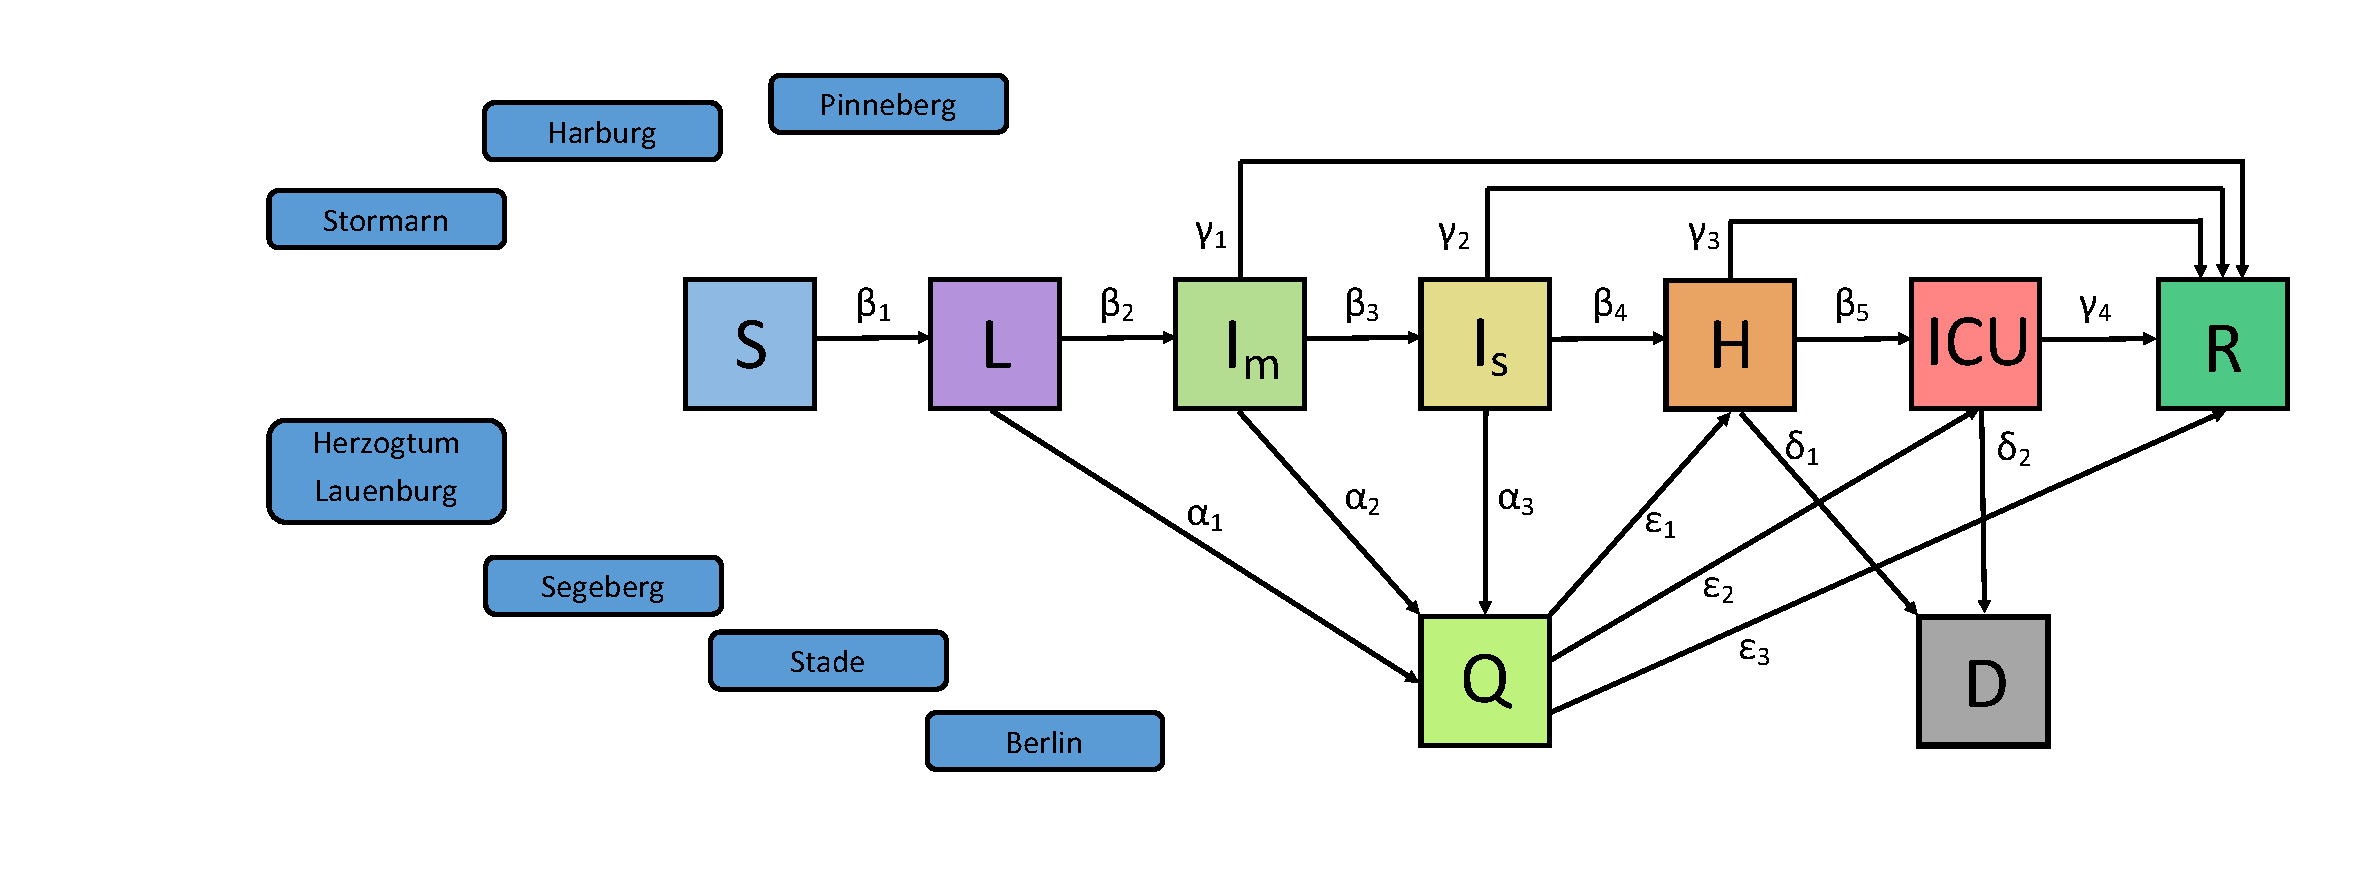
\includegraphics[width=\textwidth]{./flowchart_mit_Pendlern.pdf}
	\caption{Modell mit Pendlern.}
	\label{fig:modellPendler}
\end{figure}
%
Wir gehen davon aus, dass nur suszeptible oder latent kranke Personen zur Arbeit pendeln, alle mit Symptomen bleiben zu Hause.
\newpage
\begin{align*}
\text{kartesische Form}\quad\rightarrow\quad\begin{cases}\text{trigonometrische Form}\\
\text{Exponentialform}
\end{cases}
\end{align*}
%----------------------------------------------------------------

\begin{thebibliography}{0}
\bibitem{1} Ehmann, Katrin Zwirglmaier and Drosten, Christian and Wendtner, Clemens and Zange, MD and Vollmar, Patrick and Rosina Ehmann, DVM and Zwirglmaier, Katrin and Guggemos, MD and Seilmaier, Michael and Niemeyer, Daniela and others, \textit{Virological assessment of hospitalized cases of coronavirus disease 2019}.
%\bibitem{2} L.~Meyers, Contact network epidemiology: Bond percolation applied to infectious disease prediction and control, {\it Bulletin of the American Mathematical Society} {\bf 44.1}, (2007) 63-86.
%
\end{thebibliography}


\end{document}





